\documentclass[onecolumn, draftclsnofoot,10pt, compsoc]{IEEEtran}
\hbadness=1000 % suppress warnings
\usepackage{graphicx}
\usepackage{url}
\usepackage{setspace}
\usepackage{hyperref}
\usepackage{listings}
\usepackage{geometry}
\usepackage{longtable}
\usepackage{float}


\geometry{textheight=9.5in, textwidth=7in}

% 1. Fill in these details
\def \CapstoneTeamName{			}
\def \CapstoneTeamNumber{		69}
\def \GroupMemberOne{			Kin-Ho Lam}
<<<<<<< HEAD
\def \GroupMemberTwo{LUCIEN-ARMAND T. TAMNO}
=======
>>>>>>> 7c1d9ff65cfb8dcc035631d6a2a26c6bea86def6
\def \CapstoneProjectName{		Depth Sensing with Computer Vision and Lidar}
\def \CapstoneSponsorCompany{	Oregon State University}
\def \CapstoneSponsorPerson{	D. Kevin McGrath}


% 2. Uncomment the appropriate line below so that the document type works
\def \DocType{
	Spring Midterm Progress Report
}

\newcommand{\NameSigPair}[1]{\par
	\makebox[2.75in][r]{#1} \hfil 	\makebox[3.25in]{\makebox[2.25in]{\hrulefill} \hfill		\makebox[.75in]{\hrulefill}}
	\par\vspace{-12pt} \textit{\tiny\noindent
		\makebox[2.75in]{} \hfil		\makebox[3.25in]{\makebox[2.25in][r]{Signature} \hfill	\makebox[.75in][r]{Date}}}}
% 3. If the document is not to be signed, uncomment the RENEWcommand below
\renewcommand{\NameSigPair}[1]{#1}
\newcommand\captionof[1]{\def\@captype{#1}\caption}
%%%%%%%%%%%%%%%%%%%%%%%%%%%%%%%%%%%%%%%
\graphicspath{{images/}}
\begin{document}
	\begin{titlepage}
		\pagenumbering{gobble}
		\begin{singlespace}
			\centering
			
\includegraphics[height=4cm,natwidth=345,natheight=435]{images/osu_logo.png}
			\hfill 
			% 4. If you have a logo, use this includegraphics command to put it on the coversheet.
			%\includegraphics[height=4cm]{CompanyLogo}   
			\par\vspace{.2in}
			\centering
			\scshape{
				\huge Senior Design Capstone \DocType \par
				{\large\today}\par
				\vspace{.5in}
				\textbf{\Huge\CapstoneProjectName}\par
				\vfill
				{\large Prepared for}\par
				\Huge \CapstoneSponsorCompany\par
				\vspace{5pt}
				{\Large\NameSigPair{\CapstoneSponsorPerson}\par}
				{\large Prepared by }\par
				Group\CapstoneTeamNumber\par
				% 5. comment out the line below this one if you do not wish to name your team
				\CapstoneTeamName\par 
				\vspace{5pt}
				{\large
					\NameSigPair{\GroupMemberOne}\par
<<<<<<< HEAD
					\NameSigPair{\GroupMemberTwo}\par
=======
>>>>>>> 7c1d9ff65cfb8dcc035631d6a2a26c6bea86def6
				}
				\vspace{20pt}
			}
			\begin{abstract}  
 				Depth Sensing with Computer Vision and Lidar proposes combining computer vision and lidar to create a reliable depth sensor.
				This document details its project member's progress toward a final design.
			\end{abstract}     
		\end{singlespace}
	\end{titlepage}
\section{Table of Contents}
\tableofcontents
\bibliographystyle{IEEEtran}
\bibliography{ref}
\clearpage

\begin{singlespace}
	\section{Definitions}
		\subsection{IR}\label{def:IR}
		IR refers to the infrared light spectrum.

		\subsection{IR Depth Sensor}\label{def:depthsensor}
		A device that calculates distances by emitting infrared patterns. 
		
		\subsection{lidar}\label{def:lidar}
		Light Detection And Ranging - A method that uses lasers to measure distance
		
		\subsection{Microsoft Kinect}\label{def:kinect}
		A product that uses an IR Depth sensor to measure distances.
		Referred as a benchmark.
		
		\subsection{Logitech Brio Webcam}\label{def:brio}
		Webcam made by Logitech. \cite{logitech}
		
		\subsection{RPLidar A1}\label{def:rplidar}
		A budget lidar device made by Slamtec. \cite{slamtec}

		\subsection{Leddar M16}\label{def:m16}
		A solid-state lidar device made by Leddar. \cite{Leddartech}

		\subsection{Computer Vision }\label{def:vision}
		The methods for acquiring, processing, analyzing, and classifying digital images and extracting information.
<<<<<<< HEAD
		
			
		\subsection{Python/C API: }\label{def:API}\cite{Ctype}\par
		API: application programming interface between Python and C programs
		
		\subsection{DSCVL: }\label{def:DSCVL}
		Acronym that stands for Depth sensing with computer vision and lidar
=======
>>>>>>> 7c1d9ff65cfb8dcc035631d6a2a26c6bea86def6

		
	\section{Project Purpose}
		Infrared (IR) depth sensors such as the model used in Microsoft's Kinect \ref{def:kinect} can quickly calculate distances in indoor scenarios.
		However, IR depth sensor readings can be obfuscated by other infrared emitting sources such as other IR depth sensors or natural sunlight.
		IR depth sensors cannot be used in self-driving cars, outdoor robots, or any any device that requires high accuracy distance measurement in varying conditions.
		Depth Sensing with Computer Vision and Lidar proposes combining computer-vision image classification with lidar technology to create a robust and reliable depth sensor.

	\section{Design}
		The Logitech Brio webcam provides a high-resolution, two-dimensional image but lacks depth perception.
		The Leddar M16 provides accurate depth measurement in a horizontal dimension but lacks vertical perspective beyond a 40-degree spread.
		This project proposes bridging the utility of both devices by securing them in stationary positions, then using software to combine their outputs.		


		Figure \ref{dimensions} illustrates different dimensions measured by the M16 Lidar and Brio Webcam.
		The red cube represents the Logitech Brio webcam and M16 Lidar secured in stationary positions.
		The flat purple triangle represents the M16 Lidar's horizontal range detection.
		The transparent green rectangle in front of the person represents the computer vision model recognizing that there is a person in-front of the sensor.
		The transparent teal pyramid represents the Brio webcam's field-of-view.
		
		\begin{figure}[H]
			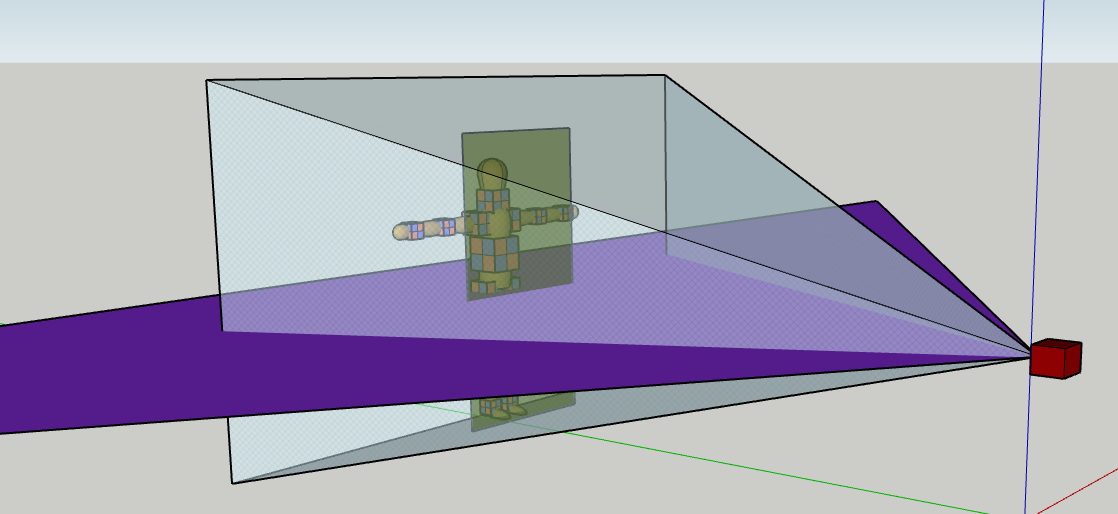
\includegraphics[scale=0.5]{different_dimensions.PNG}
			\captionof{figure}{Visualizing different dimensions measured by the M16 Lidar and Brio Webcam.}
			\label{dimensions}
		\end{figure}


	\section{Device Mount}
		Using some spare plywood, I created a mount for the Logitech Brio webcam and Leddar M16 as shown in Figure \ref{mount1}.
		This mount serves to stabilize the webcam and lidar devices in a stationary positions relative to each other so that accurate distance/visual calibrations can be performed.
		If the webcam and lidar devices are not placed in consistent positions, distance information will not be synchronized with object recognition.
		Writing an algorithm to compensate for automatic distance and object recognition calibration is an overly complex task and beyond the scope of this project.

		\begin{figure}[H]
			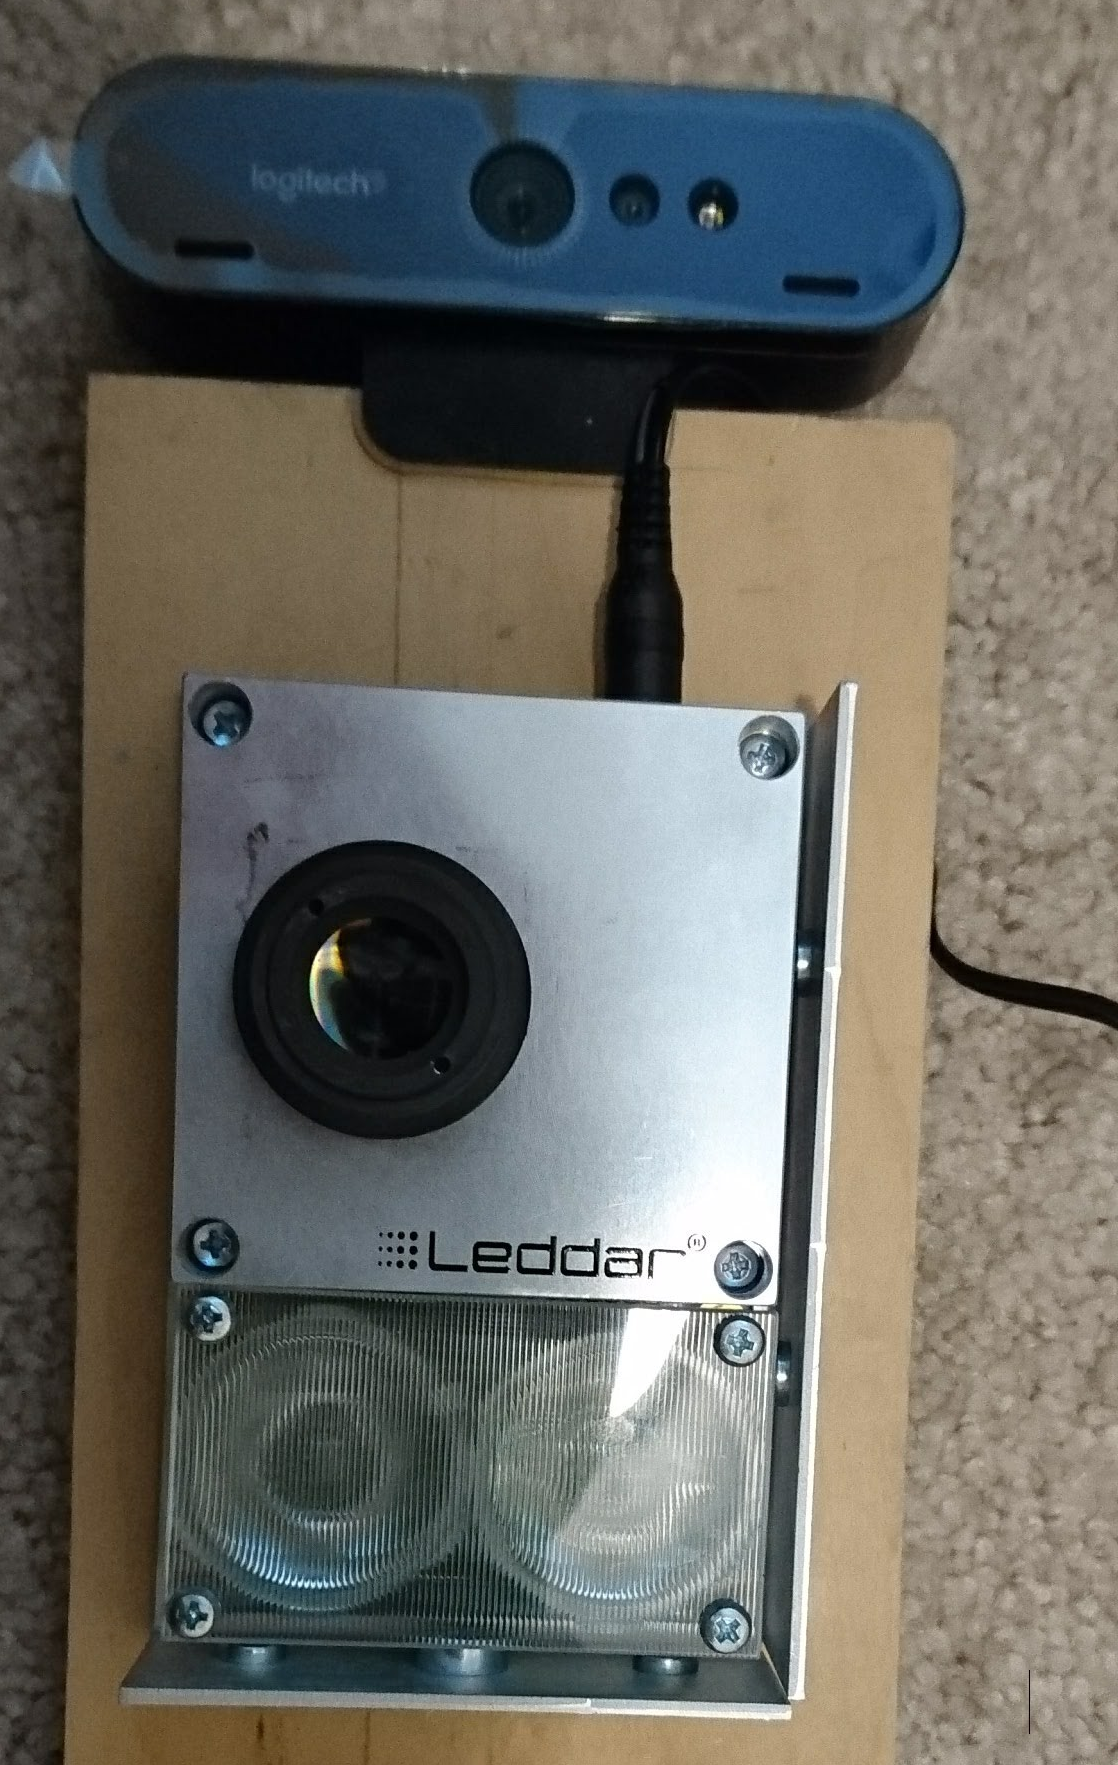
\includegraphics[scale=0.2]{mount1.PNG}
			\captionof{figure}{Part of the mount for .}
			\label{mount1}
		\end{figure}


		Progress with the Leddar M16 is slow and I do not foresee it to be working and integrated in time for expo.
		Fortunately, I was able to read distance information with the RPlidar A1.
		I adjusted the mount to accommodate the RPlidar A1 by drilling a few shallow holes in the base of the mount.
		This allows the RPlidar A1's four plastic standoffs to fit into the base of the mount as shown in Figure \ref{mount2}.

		\begin{figure}[H]
			\includegraphics[scale=0.1]{mount2.PNG}
			\captionof{figure}{Visualizing different dimensions measured by the M16 Lidar and Brio Webcam.}
			\label{mount2}
		\end{figure}

		The device mounting system is complete. 
		Our project's components can be fixed in stable positions to ensure consistent readings in different environments.
		This mounting system is important to our final design because it ensures operational consistency and simplifies the overall problem. 


		\section{Computer Vision}
			During Winter Term, I started experimenting with OpenCV's pre-trained facial/pedestrian support-vector-machine (SVM) classifier.
			This SVM is a combination of several other SVMs that detect the upper body, eyes, mouths, and noses.
			The combined SVM is intended to detect faces with high accuracy.
			However, when applied to our design, I could not consistently replicate good results.
			This was due to several factors, namely the SVM used was meant to perform classification on still images where the camera's perspective is far from the subject.
			

			Our design specifications envision a system that quickly tracks multiple subjects in a crowded expo scenario.
			In a such a scenario, human subjects will be unpredictably shifting their positions and moving in or out of the field-of-view.
			As seen in Figure \ref{svm}, the OpenCV SVM model does not perform to our specification.
			If the human subject were to turn their head or move too quickly, the SVM will have difficulty tracking their body.
			Additionally, the SVM performs intensive calculations on the computer's CPU, severely limiting the video output's frame-rate and resolution.
			
			\begin{figure}[H]
			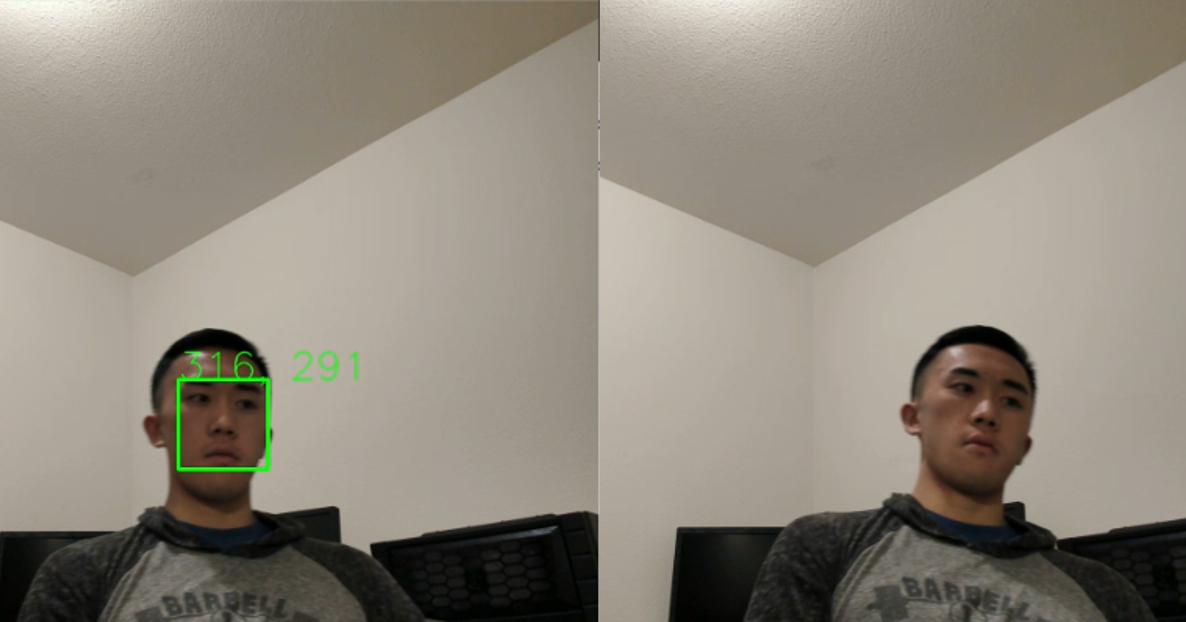
\includegraphics[scale=0.60]{svm.PNG}
			\captionof{figure}{SVM face classification (Left) fails when subject slightly turns their head (Right)}
			\label{svm}
			\end{figure}


			Tensorflow's open source object detection classifier presented a better computer-vision alternative. \cite{tensorflow}
			The Tensorflow object recognition library is better suited for this project because its library has already been trained to recognize a large dataset of objects. \cite{convolutional_object_detectors}
			These pre-trained datasets in Tensorflow's library are sourced from other machine learning datasets and employ advanced algorithms such as Single Shot Multibox Detection and Region-Based Fully Convolutional Networks. \cite{coco} \cite{open_images} \cite{kitti}


			\begin{figure}[H]
			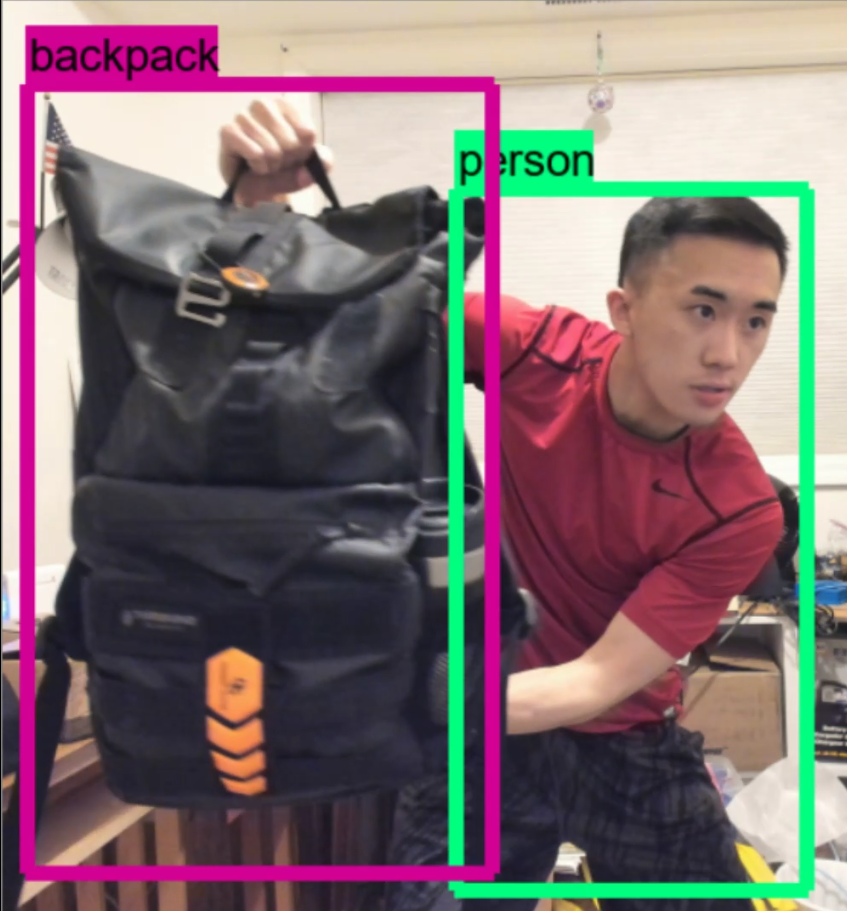
\includegraphics[scale=0.45]{tensorflow.PNG}
			\captionof{figure}{Our pre-trained Tensorflow model can  detect multiple subjects in near real-time}
			\label{tf-detect}
			\end{figure}


			Using this pre-trained Tensorflow model, our project can now accurately outline and label over 90 subjects as they come into view of the webcam.
			The current state of the code will enable us to selectively edit the output video frames to draw bounding boxes on subjects as they move in and out of the camera's field of view.


			Tensorflow also enables us to take advantage of NVIDIA CUDA, a driver that moves intensive calculations to the GPU.
			While this increases our list of material requisitions for our physical expo demo, moving calculations to the GPU greatly improves the output video quality, frame rate, resolution, and classification speed. \cite{nvidia}
			

			The computer vision aspect of our project is now complete.
			Combined with a stable mount, we now have a versatile system that can recognize over 80 distinct models such as humans, bags, or animals in near real-time.
			

	\section{Current Problems}
		\subsection{RPlidar A1 and Computer Vision Integration}
			To ensure our project will be in a presentable state by expo, I am modifying my design to use the RPlidar A1.
			Progress with the M16 lidar device has been slow, I do not foresee it being and integrated in time for expo.
			I have successfully tested the RPlidar A1 and have achieved reading some point-distance angle information.
			However, the python library used by the device calls a generator function to store its distance data.
			This type of data structure is hard to adapt for our purposes because the device's buffer will overfill and overwrite readings if it is not called fast enough.
			Figure \ref{reading} demonstrates this issue.
			To remedy this, I will experiment adjusting the loop calling the Tensorflow image recognition functions.
			I will also experiment running the RPlidar A1 in parallel with the Tensorflow image recognition.

			\begin{figure}[H]
			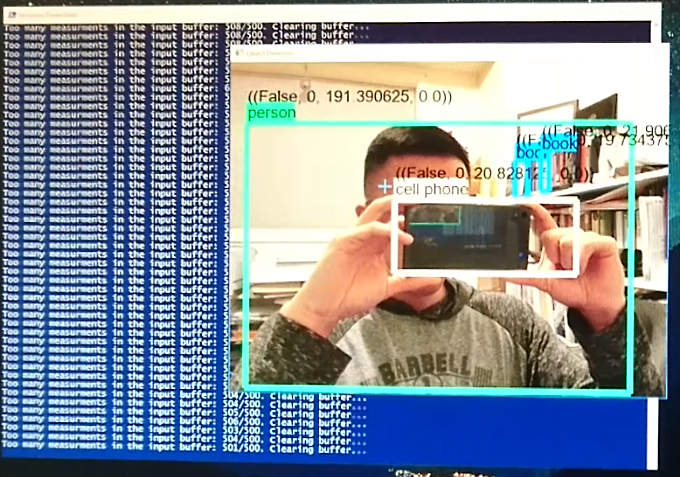
\includegraphics[scale=0.45]{reading.PNG}
			\captionof{figure}{Due to the overfilling buffer my current implementation does not calculate distances correctly.}
			\label{reading}
			\end{figure}


<<<<<<< HEAD
	
	
	\section{ Leddar M16 and Python/C API- [Constructs]---------Lucien}
				
	\section{Project Purpose}
The purpose of the DSCVL\ref{def:DSCVL} project is to come up with an effective solution of painting on a screen an image form a camera with a single point signal from another source technology called Lidar. And for the sake of DSCVL final solution accuracy and better performance,the project concept is to look for any technological tool or system that helps to build an ultimate robust software.

 In fact, on the source technology used in this project, namely the  lidar technology is known to be reliable in outdoor environment in terms of objects distance measurements, and mostly when that lidar technology uses its  16-Segment SOLID-STATE LIDAR equipment also known as the Leddar M16 \ref{def:rplidar2}. One the other hand, a webcam specifically the Logitech Brio Webcam \ref{def:brio} would help to get an image that is located right at the exact same distance than the point signal provided by the new adopted Leddar M16. All this to render with precision the object of interest whether it be a person or a liquid.
 
Moreover, the fact that the lidar technology ( Leddar M16) is much more accurate to provide better objects detection than the IR technology \ref{def:IR} in outdoor, prompts  its de facto adoption in this DSCVL project. However, it is important to know how to use this type of device, how this kind of material would fit into the entire to be built application, and ultimately how to connect the code run by the M16 to other components of the DSCVL project. \par

\section{Current State of the DSCVL}
Though, the past winter term progress report described the RPLidar A1 capability  \ref{def:rplidar} of outputting  useful information but the reality is that the DSCVL project  needed some changes for the sake of better accuracy. some changes took place at different level of the project. And the most important being the replacemnt of RPLiadr A1 by the 16 segment solid state M16 that provides better detection, localization, and distance measurements when is to compares to the RPLidar A1.\par

Additionally, those differences can even be more tangible at the code level, because the M16 model has its code literally written in C program while the RPLidar code is closely related to the python environment. And this M16 factor code-based caused me to conduct researches to figure out how can I make the C program code work in python environment. The result of that research was to discover the python \ref{Ctypes} functionality to play the intermediary role of having the C program code runs in a python environment.With the same idea, I dug a little bit more to finally find out that Visual Studio is the suitable Windows application to implement the python/C API.  

 
\subsection{ Preliminaries and the Python/C API implementation}
	\subsubsection{The default M16-Windows setting}
To stick with the Leddar M16 technology, I have to implement the python/c API\ref{def:API} using the C-code that was shipped with the M16 device. And to do so, I have to make sure first that  the M16 can properly run in a Windows environment by default. And for me to test that functionality, I installed and configured the default M16 settings, as shown in figure \ref{signal} below.

   \begin{figure}[H]
			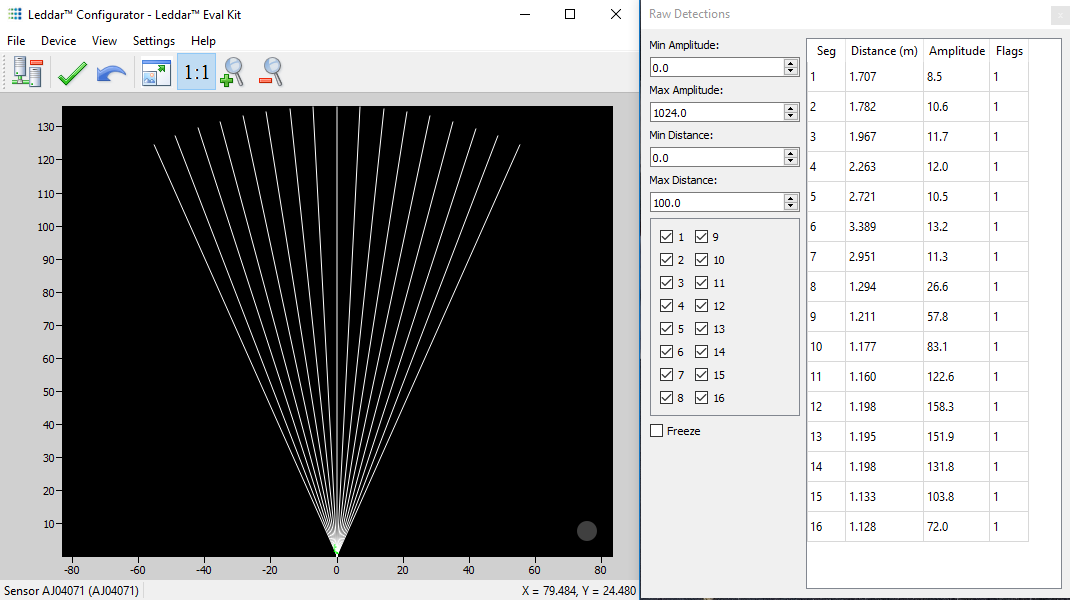
\includegraphics[scale=0.5]{images/signal.PNG}
			\caption{figure}{Leddar M16 outputs distance measurements  using the default windows installation [right] and default M16 screen [left].}
			\label{signal}
		\end{figure}
		
That figure \ref{signal} displays a sample distance outputs as it is supposed to be visualized by a user at the final stage of the DSCVL project. Though, differences may be seen in term of data disposition on the screen,because the M16 code has to run in conjunction with webcam technology to overlay images form the python environment. Hence, the implementation of the DSCVL application has an additional technological constraint to be done via an API.
		
		\subsubsection{ The Python/C API implementation, related issues and attempted solutions}
		
To get the written C language code to python, the Visual studio 2017 application appeared to be the adequate tool to use. Therefore, I installated  visual Studio in Windows 10 system, imported any necessary library to connect the visual Studio  to the Leddar M16 C-code,using the appropriate \cite{Microsoft} documentation related to the topic. 
The remaining bulk of work is  to write and debug the API implementation code to make sure the M16 interacts properly from the visual studio perspective and secondly, to integrate in a single package the python and the M16 C codes, as shown in figure \ref{C-api}.

 \begin{figure}[H]
			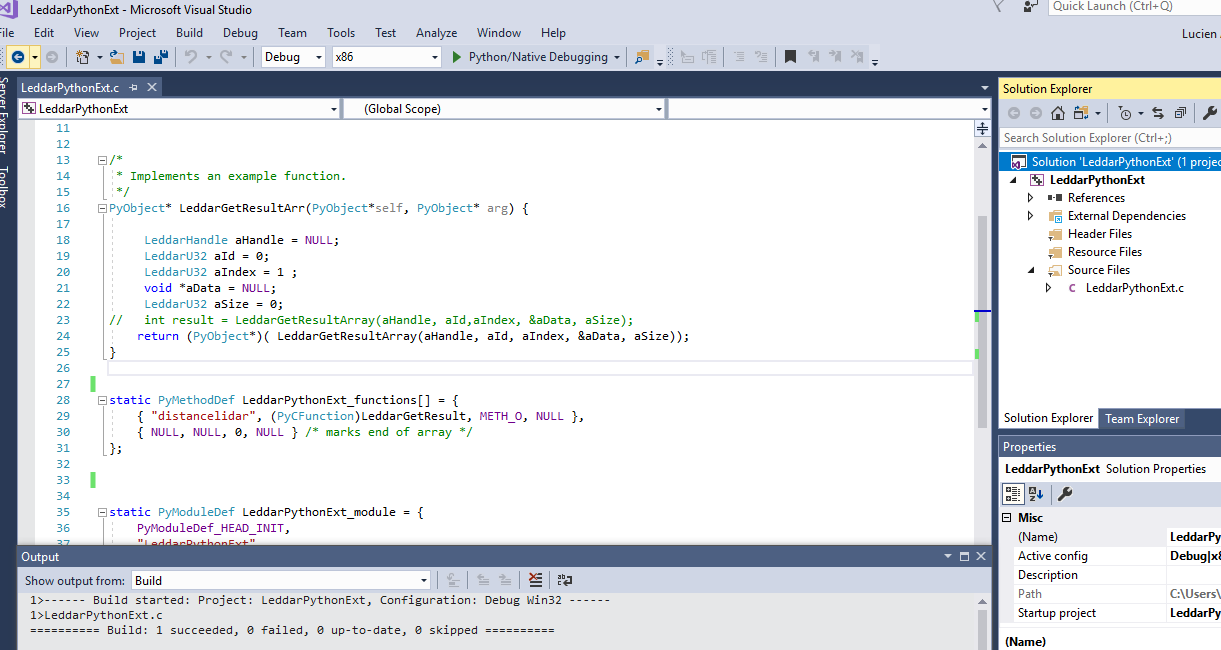
\includegraphics[scale=0.5]{images/C-api.PNG}
			\caption{figure}{Python/C API built in Visual Studio 2017.}
			\label{C-api}
		\end{figure}
		
However, when working on the  above API, I encountered multiple setbacks.among others, the two most important issues are:the slight Leddar M16  differences seen in the the M16 files, for instance I had to change one default header, as shown in figure \ref{change-M16} below.

 \begin{figure}[H]
 \centering
			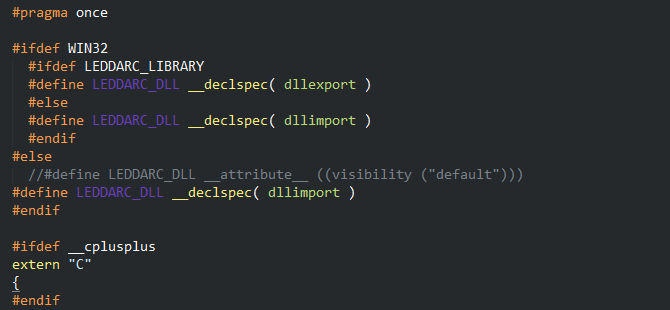
\includegraphics[scale=0.5]{images/change-M16.PNG}
			\caption{figure}{Snippet code changed in the Leddar M16 header file.}
			\label{change-M16}
		\end{figure}

And the worst being found in the current debugging phase that presents a successful result in code checker but generates several linkage errors.  

Finally, I also wrote an additional decorator function in the python module to speed up the python execution module as shown in figure \ref{change-M16}here underneath.

 \begin{figure}[H]
 \centering
			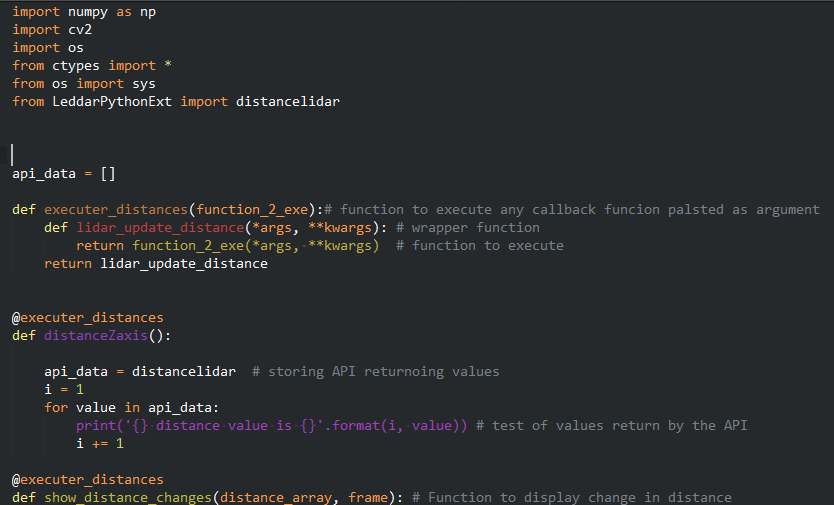
\includegraphics[scale=0.5]{images/python-code.PNG}
			\caption{figure}{Python decorators code.}
			\label{python-code}
		\end{figure}
		
		
\subsection{ Legacy: GUI Interface}

In order to prioritize the DSCVL backend, the Frontend was relegated because the backend is more important and represent the project core functionality as envisioned in the final stage. The GUI downgrade, yet still provides the basic services it has before, but it is not clear whether the final DSCVL system would make use of the legacy graphical user interface.
		
		

	\section{Conclusion}	
	This midterm progress report provides a succinct description of the work done in about a month, presents the focal point of the bulk of work that is to implement the python/C API and ultimate, problems encountered during that implementation process and finally some attempted solutions as remedy to solve those issues. 
		
=======
	\clearpage
>>>>>>> 7c1d9ff65cfb8dcc035631d6a2a26c6bea86def6

\end{singlespace}
\end{document}
